% !TEX program = xelatex
% !TeX encoding = utf8
% !TeX spellcheck = pl-PL

%%%%%%%%%%%%%%%%%%%%%%%%%%%%%%%%%%%%%%%%%%%%%%%%%%%%%%%%%%%%%%%%%%%%%%%%%%%
% Wybierz rodzaj pracy dyplomowej oraz wydział
% Pick thesis type and faculty
%%%%%%%%%%%%%%%%%%%%%%%%%%%%%%%%%%%%%%%%%%%%%%%%%%%%%%%%%%%%%%%%%%%%%%%%%%%
\documentclass[thesis=inz,faculty=ee]{EE-dyplom} 

% thesis=[inz|mgr|bsc|msc]
%  * inz - praca inżynierska
%  * mgr - praca magisterska
%  * bsc - bachelor thesis
%  * msc - master thesis

% Skróty nazw wydziałów zgodne z domenami internetowymi
% Abbreviations of Faculties according to Internet subdomains
% faculty=[
%	arch,
%	gik,
%	ee,
%	wip
%	]

%%%%%%%%%%%%%%%%%%%%%%%%%%%%%%%%%%%%%%%%%%%%%%%%%%%%%%%%%%%%%%%%%%%%%%%%%%%
% Konfiguracja - do personalizacji
% Configuration - to be personalized
%%%%%%%%%%%%%%%%%%%%%%%%%%%%%%%%%%%%%%%%%%%%%%%%%%%%%%%%%%%%%%%%%%%%%%%%%%%
\instytut{The Institute of the Theory of Electrical Engineering, Measurement and Information Systems}
\kierunek{Informatyka stosowana}
\specjalnosc{Inżynieria oprogramowania}
\title{Rozwiązanie informatyczne do organizacji korepetycji}
\engtitle{Computer solution for organizing tutoring}
\album{319052}
\author{Sebastian Kaluzinski}
\promotor{}
\date{2025}
\longdate{2025-01-25}

%\grantlicense{TRUE} % [TRUE|FALSE]

%%%%%%%%%%%%%%%%%%%%%%%%%%%%%%%%%%%%%%%%%%%%%%%%%%%%%%%%%%%%%%%%%%%%%%%%%%%
% Streszczenie pracy i abstract.
% In case of thesis in English swap the order - English version goes first.
%%%%%%%%%%%%%%%%%%%%%%%%%%%%%%%%%%%%%%%%%%%%%%%%%%%%%%%%%%%%%%%%%%%%%%%%%%%
\streszczeniepracy{
To jest streszczenie. To jest trochę za krótkie, jako że powinno zająć całą stronę.

\lipsum[1-4]
} % koniec streszczenia

\slowakluczowe{Android, Spring, Kotlin}

\thesisabstract{
This is abstract. This one is a little too short as it should occupy the whole page.

\lipsum[1-4]
} % end of abstract

\thesiskeywords{Android, Spring, Kotlin}

%%%%%%%%%%%%%%%%%%%%%%%%%%%%%%%%%%%%%%%%%%%%%%%%%%%%%%%%%%%%%%%%%%%%%%%%%%%
% Tu zaczyna się dokument
% Here is the beginning of the document
%%%%%%%%%%%%%%%%%%%%%%%%%%%%%%%%%%%%%%%%%%%%%%%%%%%%%%%%%%%%%%%%%%%%%%%%%%%
\begin{document}
    % Strony nagłówkowe
    % Headers
    \frontpages

    % Właściwa treść jest w pliku tekst/main.tex
    % Real contents is in tekst/main.tex
    % Rozdziały zaczynają się od "chapter"
\chapter*{Wstęp}
\addcontentsline{toc}{chapter}{Wstęp}
\section*{Wprowadzenie}
W wyniku dynamicznej cyfryzacji życia, przyspieszonej przez pandemię, na rynku korepetycji pojawiła się wyraźna luka.
Obecnie dostępne rozwiązania nie spełniają potrzeb użytkowników pod względem wygody zarządzania zajęciami i jakości oferowanych usług.
Brakuje narzędzia, które umożliwiłoby kompleksowe zarządzanie harmonogramem,płatnościami i komunikacją pomiędzy uczniem a korepetytorem,
co stwarza zapotrzebowanie na nowoczesną, dedykowaną aplikację.

Praca "Aplikacja mobilna do organizacji korepetycji" podejmuje implementacja podwalin do rozwijania skalowanej aplikacji mobilnej, która umożliwi uzupełnienie tej luki na powstałe na rynku.
W ramach stworzenia aplikacji zostanie zaimplementowanie zaimplementowana natywna aplikacja na system Android oraz serwer backendowy w technologii Spring Boot.
\section*{Cel pracy}
Głównym celem pracy "Implementacja aplikacji mobilnej do organizacji korepetycji" jest stworzenie aplikacji mobilnej,
która pozwoli na odpowiednia skalowanosc systemu, aby moc z latwością dodawać nowe funkcjonalności.
W przypadku serwera backendowego, celem jest stworzenie systemu, który pozwoli na zastaoswanie w przyszłości takich technologii jak mikroserwisy.
Aby zrealizować ten cel zostanie zastosowana wielo-modularna architektura, która pozwoli na latwa podmiane modułów w przyszłości na odpowiednie mikroserwisy.

W przypadku aplikacji mobilnej, celem jest stworzenie aplikacji, która pozwoli na odpowiednie odseparowanie warstw od siebie.
Będzie to osiągnięte poprzez wydzielenie odpowiednio agnostycznych interfejsów względem platformy, na której działa aplikacja.
Jest to ważne, ponieważ docelowo aplikacja ma być dostępna na systemach Android oraz iOS. Zostanie to osiągnięte poprzez zastosowanie takiej technologii jak Kotlin Multiplatform.
Dlatego niezwykle ważne jest, aby aplikacja w należyty sposób odseparowywała warstwy od siebie, aby w przyszłości móc z łatwością zastąpić warstwę widoku na odpowiednią dla systemu iOS.

\section*{Plan Pracy}


\chapter{Serwer backendowy}
W celu zaimplementowania serwera backendowego wykorzystano technologię Spring Boot.
Spring boot umożliwia szybkie tworzenie aplikacji w języku Java (jak i Kotlin), a także zapewnia wiele gotowych rozwiązań, które znacznie ułatwiają pracę.
Sprint Boot opiera się na frameworku Spring, który jest jednym z najpopularniejszych frameworków do tworzenia aplikacji backendowych.
Sam Spring wymagałby znacznie wiecje konfiguracji, co znacznie wydłużyłoby czas implementacji.
Użycie Spring Boot pozwala na skupienie się na implementacji funkcjonalności, a nie na konfiguracji,
uzycie Spring zamiast Spring Boot wymagałoby znacznie wiekszego nakładu pracy ale byłoby równie możliwe.


\section{Lista użytych technologii}
Do zaimplementowania aplikacji serwerowej zostały użyte następujące technologie, po odpowiednim porównaniu i analizie:
\begin{itemize}
    \item Java 21
    \item Gradle
    \item Kotlin
    \item JUnit
    \item Kotest
    \item Spring Boot
    \item PostgreSQL
    \item Docker-Compose
\end{itemize}
\subsection{Java 21}\label{subsec:uzyte-technologie-java}
Java 21 została użyta podczas budowania aplikacji zarówno serwerej jak i mobilnej.
Jest to spowodowane powszechnością tego środowiska co znacznie ułatwia ustawienie środowiska deweloperskiego pomiędzy róznymi systemami operacyjnymi.
Pod wezględem developmentu java nie została użyta do napisania ani jednej linijki kodu.
Język ten niesie ze sobą wiele zalet, takich jak wieloletnie wsparcie, ogromna i niezwykle aktywna społeczność, wiele poradników oraz artukułów na rozwoju projektów w tym języku.
Problemem jednak jest nullowalność, która jest w Javie ogromnym problemem.
Historycznie NullPointerExeption jest jednym z najpopularniejszym wyjątków doświadczanych przez programistów, w szczegółności Javy.
Null jest domyślną wartością każdej zmiennej w tym języku, powoduje to, że programista musi wykonywać niezliczoną ilość sanity checków, które zazwyczaj są kompletnie zbędne.
Dodatkowo powoduje to, że duża ilość kodu jest trudniejsza do odczytu.
\begin{lstlisting}[caption=Przykład obsługi null (Java)]
void someMethod(List<Item> items) {
    if (items == null) {
        throw new IllegalArgumentException("Items cannot be null");
    }

    if (items.isEmpty()) {
        throw new IllegalArgumentException("Items cannot be empty");
    }

    ...
}
\end{lstlisting}
W danym przykładzie możemy  zauwżyć, że programista został zmuszony do sprawdzenia dwóch warunków krańcowych.
Jeden z nich jest spowodowany wyłącznie przez platformę jaką jest java.
Zmienna items będącą nullem może sugerować, że lista nie została ale jednocześnie może sugerować też, że lista jest pusta.
Sytuacje tego typu powodują, że kod jest znacznie cięższy do interpretacji.
Dodatkowo nie zawsze możemy być pewni, że osoby używające naszej biblioteki będą poprawnie odróżniać kiedy null powinien być przekazywany a kiedy pusta lista.
Problemy takie mogą zostać rozwiązane przez użycie zewnętrznych bibliotek, na przykład Lombok.
Lombok pozwala na automatycznie generowanie kodu, który zazwyczaj był pisany ręcznie przez programistów.
Mowa tutaj o takich funkcjach jak gettery, settery i inne tego typu funkcjonalności, które są powtarzalne niezależnie od kontektu występowania.
\begin{lstlisting}[caption=Przykład obsługi null (Java z Lombok)]
void someMethod(@NonNull List<Item> items) {
    if (items.isEmpty()) {
        throw new IllegalArgumentException("Items cannot be empty");
    }

    ...
}
\end{lstlisting}
W powyższym przykładzie została użyta adnotacja @NotNull, która automatycznie generuje sanity check dla pola, które zostało oznaczone tą adnotacją.
Powyższy kod jest czytelniejszy i nie wymaga sprawdzenia czy przekazywana zmienna jest nullem, jednak nie pozbywamy się problemu nullowalności.
Jedynie zwiększamy czytelność kodu, adnotacja wygenerowała automatycznie kod, który wykonuje to sprawdzenie zamiast programisty.
W rzeczywistości kod z przykładu numer 2 jest identyczny z kodem z przykładu numer 1, jedynie pierwszy warunek został automatycznie wygenerowany przez Lombok.

\begin{lstlisting}[caption=Przykład w języku Kotlin]
fun someMethod(items: List<Item>) {
    require(items.isNotEmpty()) { "Items cannot be empty" }

    ...
}
\end{lstlisting}
Powyższy przykład demonstruje prawie równoznaczny kod w języku Kotlin, największą różnicą jest to, że zmienna "items" nie może być nullem.
Kotlin nie pozwala na niejawne przekazanie nulli, co znacząco eliminuje problem rozgałęzień w logice jeśli nie jest to wymagane przez logikę biznesową.
\begin{lstlisting}[caption=Przykład w języku Kotlin]
fun someMethod(items: List<Item>?) {
    if (items == null) {
        throw IllegalArgumentException("Items cannot be null")
    }

    if (items.isEmpty()) {
        throw IllegalArgumentException("Items cannot be empty")
    }
    ...
}
\end{lstlisting}
Powyższy przykład pokazuje równoznaczy kod w języku kotlin do Javy z przykładu numer 1.
Dużą różnicą jest to, że w kotlinie zmienna nie może posiadać wartości null jeśli nie jest to jawnie zadeklarowane.
Znacznie ulepsza to czytelność kodu oraz wymusza użytkownika narzędzi do przekazywania list z odpowiednią wartością.
Powoduje to, że kod jest znacznie bardziej czytelny oraz łatwiejszy do zrozumienia.
\subsection{Gradle}\label{subsec:uzyte-technologie-gradle}
Jako narzędzie do budowania projektu oraz zarządzania wybrałem Gradle.
Dużą zaletą w porównaniu do Maven jest deklaratywność w definiowaniu zależności oraz konfiguracji projektu.
Maven jest oparty na instrucjach, Gradle jest oparty na deklaracjach.
\cite{mavenDefinitiveGuide}
\cite{gradleForAndroid}
W aplikacji serwerowej zależało mi na możliwości automatyzacji wielu procesów związanych z budowaniem projektu oraz lepszego śledzenia zależności między modułami.
Gradle pozwala na zbudowanie drzewa zależności pokazującego jakie moduły zależą od siebie.
Przykładowe drzewo zależności dla projektu Android pt. \href{https://github.com/savvasdalkitsis/module-dependency-graph?tab=readme-ov-file}{} Game Frame
\begin{figure}[H]
    \centering
    \clearpage
    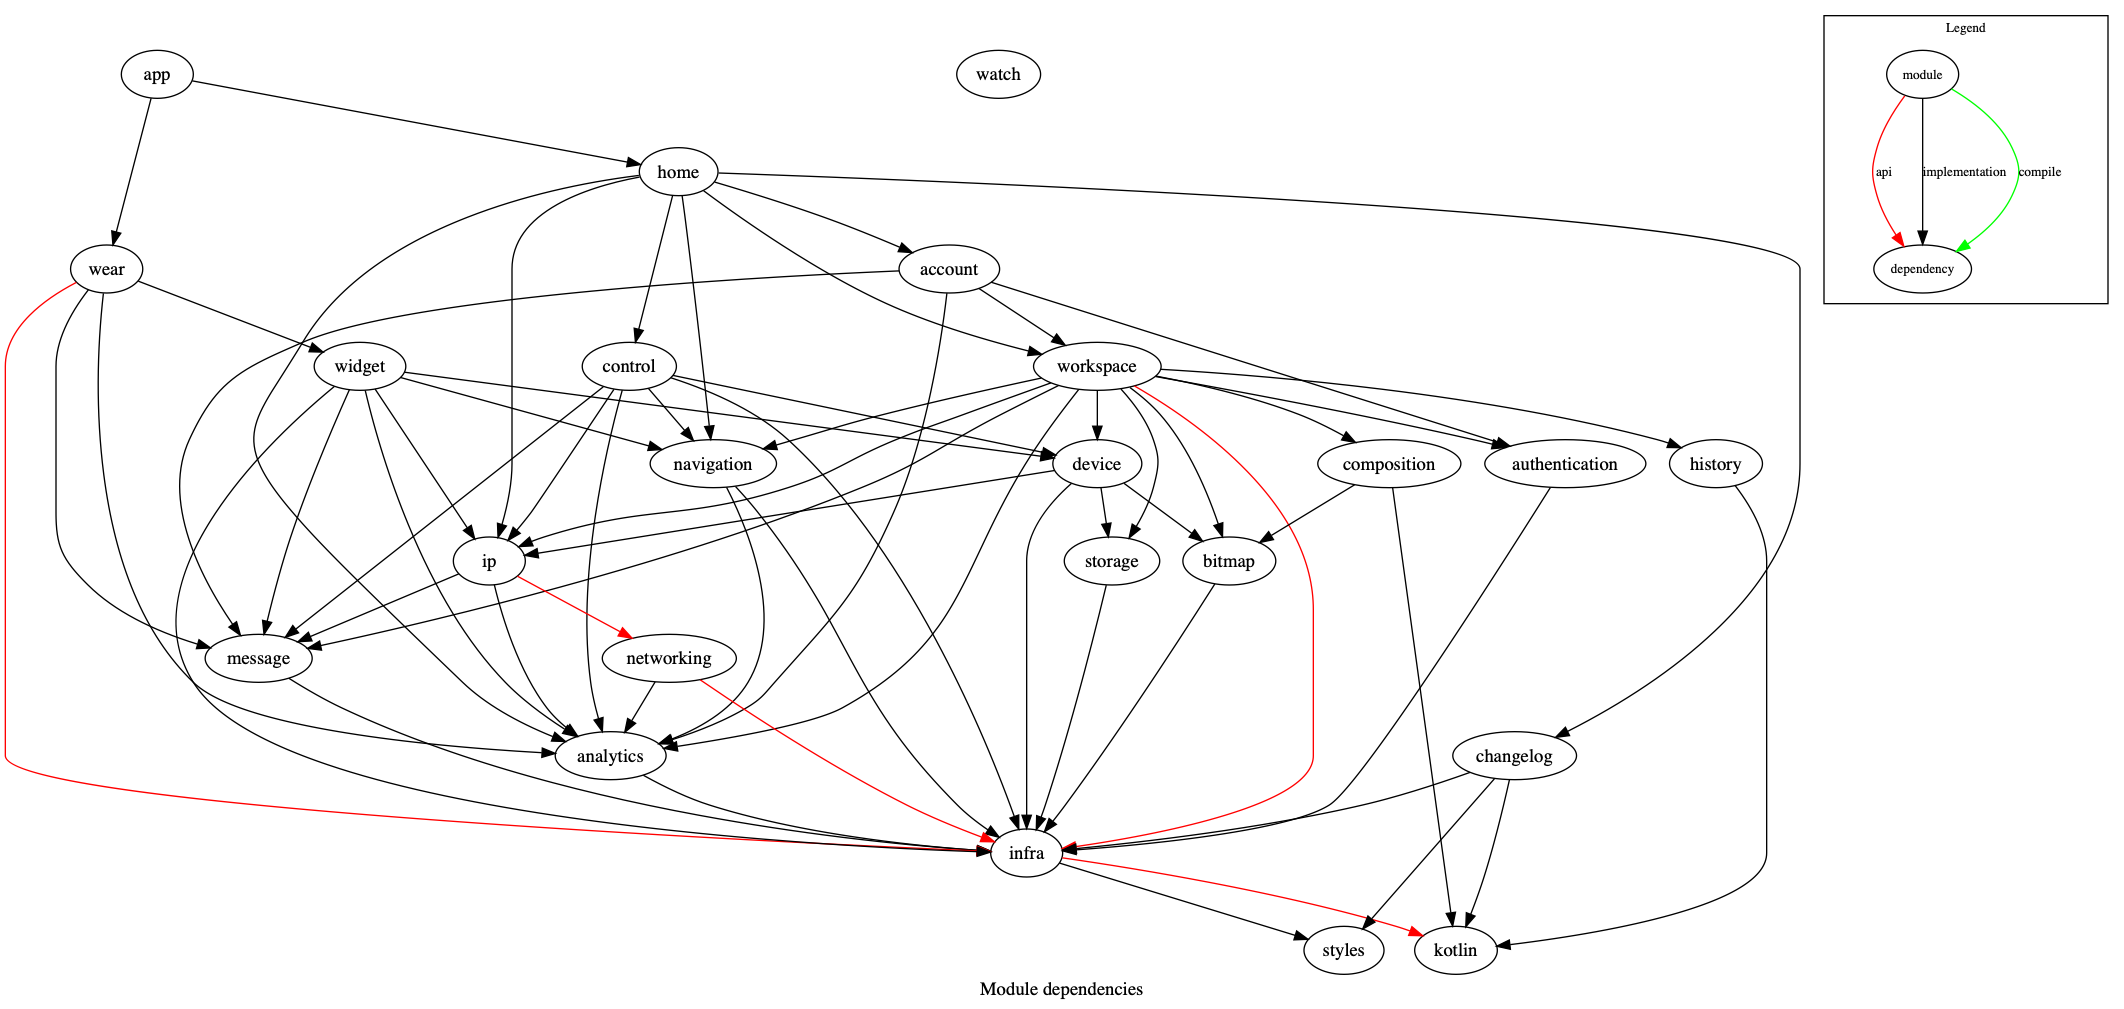
\includegraphics[width=15cm,keepaspectratio]{rysunki/module_graph.png}
    \caption{Przykładowe drzewo zależności w projekcie Game Frame, źródło: https://github.com/savvasdalkitsis/module-dependency-graph?tab=readme-ov-file}
    \label{fig:gameframe-deps-tree}
\end{figure}
Dodatkowo możliwe jest szybkie napisanie pluginu, który pozwoliłby na zbadanie bibliotek, frameworków oraz innych zależności używanych w projekcie przez wszystkie moduły pod kątem znalezienia części wspólnej.
Również niezwykle przydatną funkcjonalnością gradle jest możliwość zbudowania drzewa zależności w ramach jednego modułu.
\cite{gradleDepsTree}
\begin{figure}[H]
    \centering
    \clearpage
    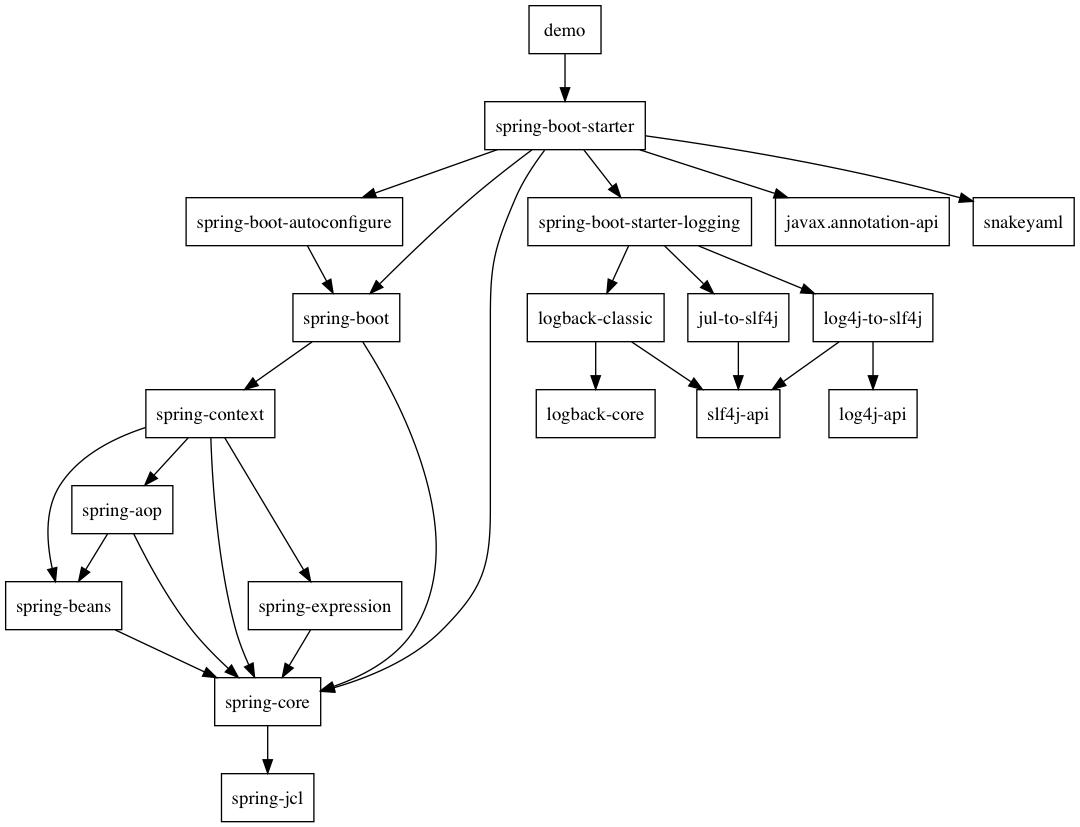
\includegraphics[width=10cm,keepaspectratio]{rysunki/gradle-deps-tree.png}
    \caption{Przykładowe drzewo zależności w module, źródło: https://blog.droidchef.dev/mastering-the-gradle-dependency-tree/}
    \label{fig:module-deps-tree}
\end{figure}

\subsection{Kotlin}\label{subsec:uzyte-technologie-kotlin}
Do samej implementacji aplikacji serwerowej wybrałem język Kotlin jako główny język programowania.
Kotlin jest językiem wspierający zarówno paradygmaty programowania obiektowego jak i funkcyjnego, jednocześnie jest w pełni interoperacyjny z Javą.
Pozwala to na stopniowe przechodzenie z Javy na Kotlin w projektach z znacznie większym długiem technologicznym.
Dodatkowo Kotlin pozwala na swobodne wywołanie kodu Javy wewnątrz Kotlina, pozwala to na łatwe wykorzystanie dotychczasowego zbioru bibliotek napisanych w Javie.
Frameworki czy też biblioteki dotychczas pisane do użytku w projektach Javowych mogą więc być używane w projektach Kotlinowych bez konieczności ich przepisywania.
Przykładem takiej biblioteki jest Spring, jeden z najpopularniejszych frameworków do tworzenia aplikacji backendowych na świecie.
Dużą zaletą Kotlina jest silne typowanie jak i brak domyślnej wartości null kryjącej się pod każdą zmienną.
Dodatkowo język pozwala na wiele uproszczeń składniowych, które znacznie ułatwiają pisanie kodu czy też wiele ułatwień slużących do łatwiejszej interakcji z kodem, nad którym nie mamy kontroli.
Przykładem tego mogą być extension functions, które pozwalają na dodanie nowych funkcji do istniejących klas, bez konieczności dziedziczenia po nich lub extension properties, które pozwalają na dodanie dodatkowych pół.
Załózmy, że zewnętrzna biblioteka zwraca nam klasę, która odwzorowuje użytkownika.
\begin{lstlisting}[caption=Przykład klasy User w Javie]
public class User {
    private String name;
    private String surname;
    private LocalDateTime birthDate;

    public User(String name, String surname, LocalDateTime birthDate) {
        this.name = name;
        this.surname = surname;
        this.birthDate = birthDate;
    }
}
\end{lstlisting}
Chcemy dodać do tej klasy funkcję, która sprawdzi czy dany użytkownik jest uprawniony do głosowania w danym kraju, dodatkowo chcemy zwrócić informację o tym czy użytkownik jest powyżej 18 roku życia.
Załóżmy, że chcemy tą klasę rozszerzyć o kilka funkcjonalności potrzebnych nam w naszym projekcie bez konieczności zmiany kodu źródłowego tej klasy:
\begin{itemize}
    \item funkcja, która sprawdzi czy użytkownik jest uprawniony do głosowania w danym kraju
    \item pole, które zwróci wiek użytkownika
    \item pole, które zwróci czy użytkownik jest powyżej 18 roku życia
\end{itemize}

\begin{lstlisting}[caption=Extension function sprawdzające czy użytkownik jest uprawniony do głosowania w w danym kraju]
fun User.canVote(country: Locale): Boolean {
    val votingAge = when (country) {
        Locale.US -> 18
        Locale.UK -> 18
        Locale.GERMANY -> 16
        else -> 18
    }
    return age >= votingAge
}
\end{lstlisting}

\begin{lstlisting}[caption=Extension property zwracające wiek użytkownika]
val User.age: Int
    get() = Period.between(birthDate.toLocalDate(), LocalDate.now()).years
\end{lstlisting}

\begin{lstlisting}[caption=Extension property zwracające czy użytkownik jest powyżej 18 roku życia]
val User.isAdult: Boolean
    get() = age >= 18
\end{lstlisting}

\begin{lstlisting}[caption=Przykład użycia extension functions]
val user = User("Jan", "Kowalski", LocalDateTime.of(2000, 1, 1, 0, 0))
val isAdult = user.isAdult
val canVote = user.canVote(Locale.US)
println("Is user adult: $isAdult, can vote: $canVote")
\end{lstlisting}
\begin{lstlisting}[caption=Wynik]
Is user adult: true, can vote: true
\end{lstlisting}
Dodatkową zaletą w porównaniu do Javy jest strukturalna współbieżność, pozwala ona na prostsze tworzenie wielowątkowych aplikacji.
\cite{structuredConcurrency}
Hierarchiczna struktura, która jest wymuszona dla zadań współbieżnych sprawia, że jako programista nie musimy zarządzać anulowaniem zadań w ramach zdefiniowanego zakresu współbieżności.
Korutyny w Kotlinie pozwalają na tworzenie zadań współbieżnych, które są zarządzane przez strukturę, która je stworzyła.\cite{effectiveKotlin}
Zakres korutyn zarządza ich cyklem życia, w przypadku anulowania zakresu, wszystkie korutyny wewnątrz niego dostają sygnał do zakończenia swojego działania dzięki propagacji anulowania w górę hierarchii.
Propagacja wydarzeń w zakresie korutyn pozwala uniknąć wycieków pamięci czy też innych problemów związanych z zarządzaniem zadaniami współbieżnymi.
\begin{lstlisting}[caption=Przykład korutyny w Kotlinie]
runBlocking {
    println("Program starts")

    val parentJob = launch { // Parent scope
        val childJob1 = launch { // Child scope
            repeat(5) { i ->
                println("Child 1: Doing work $i")
                delay(500)
            }
        }

        val childJob2 = launch { // Child scope
            repeat(5) { i ->
                println("Child 2: Doing work $i")
                delay(500)
            }
        }

        delay(1200) // Parent scope waits for 1.2 seconds
        println("Parent coroutine: Cancelling all children")
        cancel() // Cancelling parent scope cancels all children
    }

    parentJob.join() // Wait for parent job to finish
    println("Program ends")
}
\end{lstlisting}
\begin{lstlisting}[caption=Wynik]
Program starts
Child 1: Doing work 0
Child 2: Doing work 0
Child 1: Doing work 1
Child 2: Doing work 1
Child 1: Doing work 2
Child 2: Doing work 2
Parent coroutine: Cancelling all children
Program ends
\end{lstlisting}
\subsection{JUnit}\label{subsec:uzyte-technologie-junit}
Jeśli chodzi o testowanie aplikacji serwerowej, wybrałem JUnit jako framework do testów jednostkowych.
Jest to jeden z najpopularniejszych frameworków, prawdopodobnie najpopularniejszy w języku Java.

\subsection{Kotest}\label{subsec:uzyte-technologie-kotest}
Kotest jest również frameworkiem do testów jednostkowych, jego główną zaletą jest deklaratywność w porównaniu do JUnit.
Biblioteka ta pozwala na testowanie zależności między warstwami kodu.
Przykładem może być testowanie tego czy przypadkiem klasa z warstwy domenowej nie polega na klasach z warstwy obsługi zapytań użytkownika.
\begin{lstlisting}[caption=Przykład testu w Kotest]
@Test
fun `domain classes should not depend on rooting classes`() {
    val forbiddenPackage = "com.example.ui"
    val rootingClasses = getClassesInPackage("com.example.rooting")

    rootingClasses.forEach { clazz ->
        val imports = clazz.getImportedClasses()
        val domainDependsOnRooting = imports.any { it.startsWith(forbiddenPackage) }

        assertFalse(domainDependsOnRooting) { "${clazz.simpleName} depends on UI classes" }
    }
}
\end{lstlisting}

\subsection{Spring Boot}\label{subsec:uzyte-technologie-spring-boot}
Wybrałem Spring Boot jako framework do implementacji aplikacji serwerowej zamiast tradycyjnego Springa z powodu jego prostoty w konfiguracji.
Czysty Spring pozwala na znacznie większą kontrolę nad funkcjonalnościami i samym działaniem aplikacji, jednak wiąże to się z ogromnym narzutem ilości konfiguracji.
Wybranie czystego Springa zamiast Spring Boota wymagałoby znacznie większego nakładu pracy.
W aktualnym projekcie zależało mi na skalowalności oraz łatwości utrzymaniam, dlatego wybrałem Spring Boot.
Sama zamiana Spring Boota na Springa nie byłaby problematyczna dzięki architekturze aplikacji.
Wielomodularny monolit, który został zaimplementowany pozwala na łatwą podmianę frameworka tylko w jednym module.

\subsection{PostgreSQL}\label{subsec:uzyte-technologie-postgresql}
Jako bazę danych wybrałem PostgreSQL.
Jest to jedna z najpopularniejszych baz danych open-source na świecie, jego prostota w konfiguracji, ogromna ilość dokumentacji oraz szybkość działania sprawiają, że nie rozważałem innych rozwiązań.
PostgreSQL pozwala na łatwe skalowanie, zarówno wertykalne jak i horyzontalne.
Jeśli mowa o horyzontalnym skalowanie to wystarczyłoby użyć takich praktyk jak sharding lub replikacja.
Sharding pozwala na podzielenie bazy danych na mniejsze części, które są przechowywane na różnych serwerach.
W przypadku skalowania wertykalnego, PostgreSQL pozwala na monitorowanie najbardziej kosztownych zapitań, automatyczne partycjonowanie, automatyczną kompresję oraz wiele innych funkcji, które pozwalają na zwiększenie wydajności bazy danych.

\subsection{Docker-Compose}\label{subsec:uzyte-technologie-docker-compose}
Do konteneryzacji aplikacji serwerowej wybrałem Docker-Compose.
Docker-Compose pozwala na łatwe zarządzanie wieloma kontenerami jednocześnie.
Użycie Docker-Compose pozwoliło mi na łatwe uruchomienie bazy danych, aplikacji serwerowej oraz innych usług, które były potrzebne do działania aplikacji niezależnie od systemu operacyjnego.
Było to znacznym ułatwieniem w czasie developmentu zarówno przy użyciu systemu Windows jak i Ubuntu.
\cite{postgresSharding}


\chapter{Aplikacja mobilna}
Głównym celem w czasie implementacji aplikacji mobilnej była implementacja aplikacji używającej odpowiednich praktyk programistycznego tworzenia aplikacji mobilnych takich jak:
\begin{itemize}
    \item[--] architektura MVVM,
    \item[--] odpowiednie odseparowanie warstw od siebie,
    \item[--] wykorzystanie podglądów ui bez konieczności uruchamiania aplikacji,
    \item[--] wykorzystanie takich podejść jak Unidirectional Data Flow, Dependency Injection, Reactive Programming.
\end{itemize}
Najważniejszym aspektem z wyżej wymienionych było odpowiednie odseparowanie warstw od siebie.
Jest to ważne z tego względu, że użycie technologii Kotlin Multiplatform będzie niezwykle ciężkie do zrealizowania w sytuacji, gdy w klasach, które mają być współdzielone, będą znajdować się zależności od konkretnych platform.
Przykładem tego może być klasa odpowiedzialna za pobieranie danych z internetu.
Jeżeli w tej klasie umieścimy zależności należące tylko do androida tak jak np \texttt{android.content.Context}, to nie będzie możliwe użycie tej klasy w kodzie współdzielonym do momentu refaktoryzacji.

\section{Lista użytych technologii}
\subsubsection{Kotlin}\label{app:used_technologies:kotlin}
Aplikacja mobilna została w całości zaimplementowana z pomocą języka programowania Kotlin.
Kotlin został oficjalnie wybrany przez Google jako preferowany język programowania dla aplikacji mobilnych na platformę Android 7 maja 2019 roku.
\cite{kotlinWikipedia}
W przypadku aplikacji mobilnej wybranie Javy zamiast Kotlina skutkowałoby w byciu zmuszonym do imperatywnego frameworka do tworzenia widoków.
Java nie pozwala na użycie deklaratywnego frameworka oraz ten język nie jest już rozwijany przez Google od wielu lat.
Z tego powodu wybranie Javy skutkowałoby w przyszłym "tech debt".
W momencie pisania aplikacji tworzylibyśmy kod, który staje się obciążeniem i problemem w przyszłości od momentu wytworzenia go.
Użycie technologii, która nie jest rozwijana i będzie wymagała przepisania możemy uznać za źródło długu wdrożeniowego.
\cite{legacyDebt}
Rozwijanie nowego projektu z już obecnym długiem technologicznym jest równoznaczne z zaciągnięciem długu technologicznego, który będzie musiał zostać spłacony w przyszłości.
Dług technologiczny (ang. technical debt) jest terminem używanym do opisania różnicy między aktualnym stanem naszego rozwiązania a idealnym stanem, do którego powinno się dążyć w celu uzyskania skalowanego produktu, który jest łatwy w utrzymaniu.
\cite{techDebtAccerelate}

\subsection{Compose}\label{app:used_technologies:compose}
Compose to deklaratywny framework do tworzenia interfejsów użytkownika w języku Kotlin.
Deklaratywność pozwala skupić się programiście na opisaniu zachowania interfejsu zamiast skupiania się na manipulacji samym wyglądem interfejsu.
W przeciwieństwie do imperatywnego podejścia, które było preferowanym sposobu tworzenia interfejsu przez ponad 13 lat, compose wymaga odpowiedniego oddzielenia stanu od widoku.
Framework ten działa na podstawie tworzenia drzewa widoków, które jest renderowane na ekranie.
\cite{composeTree}
W momencie kiedy zmienia się wartość przekazywana jako parametr do widoku, framework automatycznie przerysowuje widok.
Sytuację tą nazywamy rekompozycją.
\cite{composeRecomposition}
Framework decyduje czy należy wykonać rekompozycję na podstawie zmiany wartości przekazywanej do widoku, która jest sprawdzana za pomocą metody \texttt{equals}.
Dlatego ważne jest aby przekazywać do widoków jak najprostsze obiekty.
Każde porównanie wartości przekazywanych ma swój koszt obliczeniowy.
Im bardziej złożony obiekt przekazujemy do widoku, tym więcej czasu zajmie porównanie go z poprzednią wartością.
Pojedyńcze obiekty stanowiłyby problemu, jednak w sytuacji gdy nasza aplikacja miałaby dziesiątki widoków, które musiałyby sprawdzać obiekty będące boskimi obiektami (ang. god objects), mogłoby to spowodować spadek wydajności aplikacji.
\cite{godObjectWikipedia}
Wymusza to na programiście odpowiednie rozdzielenie stanu danej części aplikacji od innych części, przekazywanie wcześniej wymienionych boskich obiektów do rożnych części aplikacji powodoałoby konieczność rekompozycji całej aplikacji.
Można to zoobrazować na przykładzie sytuacji kiedy zmiana wpisanego tekstu w formularzu powoduje konieczność ponownego obliczenia całego drzewa widoków.
Dodatkowo framework ten opiera się na paradygmacie kompozycji zamiast dziedziczenia.
W przypadku androida, dziedziczenie widoków było jednym z największych problemów, które wraz z czasem urosły do nieprzewidywalnych rozmiarów.
Każdy widok dziedziczył po klasie \texttt{View}, co powodowało, że każdy widok również dziedziczył problemy występujące pośród 40 tysięcy linii kodu.
Wraz z czasem pojawiały się problemy, które zostały zignorowane przez firmy tworzące swoje nakładki na androida.
Rozwiązanie problemów występujące na oryginalnej platformie w połączeniu z problemami występującymi na nakładkach powodowały, że systemy stawały się coraz bardziej niestabilne i trudniejsze w utrzymaniu.
Aby zaimplementować prostą listę elementów w XMLu, programista musiał zaimplementować dziedziczenie po klasie \texttt{ListView}, która dziedziczyła po klasie \texttt{ViewGroup}, która dziedziczyła po klasie \texttt{View}.
Dodatkowo trzeba stworzyć odpowiedni adapter, który będzie odpowiedzialny za przekazywanie danych do widoku.
Finalnie trzeba przypisać adapter do widoku, zaaktualizować widok i przekazać dane do adaptera.
Przykład widoku:
\begin{lstlisting}[language=xml]
    <FrameLayout
        android:layout_width="match_parent"
        android:layout_height="match_parent">
        <androidx.recyclerview.widget.RecyclerView
    android:id="@+id/recyclerView"
    android:layout_width="match_parent"
    android:layout_height="match_parent"
    tools:listitem="@layout/item_layout" />
    </FrameLayout>
\end{lstlisting}
Przykład implementacji pojedyńczego widoku w liście:
\begin{lstlisting}[language=xml]
<TextView
    android:id="@+id/itemText"
    android:layout_width="match_parent"
    android:layout_height="wrap_content"
    android:padding="16dp"
    android:textSize="16sp" />
\end{lstlisting}
Przykład implementacji adaptera:
\begin{lstlisting}[language=Kotlin]
class ItemAdapter(private val items: List<Item>) : RecyclerView.Adapter<ItemAdapter.ItemViewHolder>() {
    override fun onCreateViewHolder(parent: ViewGroup, viewType: Int): ItemViewHolder {
        val view = LayoutInflater.from(parent.context).inflate(R.layout.item_layout, parent, false)
        return ItemViewHolder(view)
    }

    override fun onBindViewHolder(holder: ItemViewHolder, position: Int) {
        holder.bind(items[position])
    }

    override fun getItemCount(): Int = items.size

    class ItemViewHolder(itemView: View) : RecyclerView.ViewHolder(itemView) {
        private val itemText: TextView = itemView.findViewById(R.id.itemText)

        fun bind(item: Item) {
            itemText.text = item.text
        }
    }
}
\end{lstlisting}
Finalnie należy przypisać adapter do widoku:
\begin{lstlisting}[language=Kotlin]
class MainActivity : AppCompatActivity() {
    override fun onCreate(savedInstanceState: Bundle?) {
        super.onCreate(savedInstanceState)
        setContentView(R.layout.activity_main)

        val recyclerView: RecyclerView = findViewById(R.id.recyclerView)
        recyclerView.layoutManager = LinearLayoutManager(this)

        val items = listOf(Item("Item 1"), Item("Item 2"), Item("Item 3"))
        recyclerView.adapter = ItemAdapter(items)
    }
}
\end{lstlisting}
Równoznaczny kod w compose do utworzenia widoku
\begin{lstlisting}[language=Kotlin]
@Composable
fun ItemList(
    myItems: List<Item>
) {
    Column {
        myItems.forEach { item ->
            Text(text = item.text)
        }
    }
}
\end{lstlisting}
Przypisanie widoku do aktywności aplikacji:
\begin{lstlisting}[language=Kotlin]
class MainActivity : AppCompatActivity() {
    override fun onCreate(savedInstanceState: Bundle?) {
        super.onCreate(savedInstanceState)
        setContent {
            val items = listOf(Item("Item 1"), Item("Item 2"), Item("Item 3"))
            ItemList(items)
        }
    }
}
\end{lstlisting}
Dodatkowym plusem jest to, że całośc rozwoju aplikacji odbywa się w jednym języku programowania.
Sztuczna inteligencja w IDE pozwala na szybkie i sprawne podpowiedzi, które znacznie przyspieszają proces tworzenia aplikacji.
\subsection{Koin}\label{app:used_technologies:koin}
Do wstrzykiwania zależności w aplikacji został użyty framework Koin.
Jest on biblioteką, która pozwala na wstrzykiwanie zależności w sposób deklaratywny, dodatkowo jest możliwa do wykorzystania w przypadku aplikacji androidowych, backendowych, desktopowych oraz wieloplatformowych.
Pozwala to na przygotowanie aplikacji, która może być łatwo przenoszona między różnymi platformami.
Dzięki temu przygotowaniu wystarczyłoby zmienić implementację danego interfejsu odpowiednio dla platformy, a cała reszta aplikacji pozostałaby bez zmian.
\cite{koinMultiplatform}

\subsubsection{Ktor}\label{app:used_technologies:ktor}
Ktor jest biblioteką do tworzenia serwerów HTTP w języku Kotlin oraz klientów HTTP.
Użycie tej biblioteki pozwala uniknąć potrzeby przepisywania kodu w sytuacji chęci uczynienia z aplikacji natywnej aplikację wieloplatformową.
Pozwala to na wykorzystanie napisanego kodu na aplikację androidową jako wspólny kod dla aplikacji wieloplatformowej.
\cite{ktorMultiplatform}



    % Bibliografia - musi być
    % Bibliography - must exist
    \bibliografia

    % Strony końcowe - można zakomentować, jeśli zbędne
    % Additional pages - comment out if not needed
    
    % Wykaz symboli i skrótów - patrz opis w tekście przykładowym
%    \acronymslist
%    % Spis rysunków
%    \listoffigures
%    % Spis tabel
%    \listoftables
%    % Załączniki (plik appendices.tex)
%    \easyappendices
\end{document}
%%%%%%%%%%%%%%%%%%%%%%%%%%%%%%%%%%%%%%%%%%%%%%%%%%%%%%%%%%%%%%%%%%%%%%%%%%%

